\documentclass{beamer}

\title{The Political Psychology of State Repression}
\subtitle{A Replication Exercise}
\author{Haseeb Bajwa, Rithika Kumar, John Matthews}

\begin{document}
\frame {
		\titlepage
	}
	\frame {
		\frametitle{Experiment}
		\begin{itemize}
		    \item How does fear affect the level of dissent in people’s behavior
		    \item Respondents were asked to reflect upon and describe a situation that makes them relaxed (control) or afraid (treatment) in detail and in a way that would make another individual feel the emotion.(Affective Emotional Memory Task)
		    \item Half of respondents were asked to describe political fears, other half to describe non-political fears
		    \item Respondents were asked a series of 12 questions on their propensity to participate in dissent
		    \item Also given a wristband with a pro-democracy slogan or another plain wristband as a gift for participating in the study (behavioral measure)
		\end{itemize}
	}
    \frame{
        \frametitle{Summary Statistics}
        \begin{table}[ht]
\label{summarybal}
\caption{Summary Statistics and Balance on Baseline Covariates}
\centering
\scalebox{.7}{\begin{tabular}{rrrrrrrr}
  \hline
   & \multicolumn{3}{c}{\textit{Mean}} & \multicolumn{2}{c}{\textit{Difference}}& \multicolumn{2}{c}{\textit{p-value}}\\ 
\cline{2-4} \cline{5-6} \cline{7-8} 
\\[-4.8ex]  \\ 
 & C & T_{GF} & T_{PF} & T_{GF} - C & T_{PF} - C & T_{GF} - C & T_{PF} - C \\ 
  \hline
Female & 0.53 & 0.51 & 0.51 & 0.02 & 0.02 & 0.72 & 0.71 \\ 
  Education (4-pt scale) & 1.74 & 1.65 & 1.74 & 0.09 & -0.00 & 0.18 & 0.98 \\ 
  Age & 37.74 & 37.92 & 37.95 & -0.18 & -0.21 & 0.89 & 0.87 \\ 
  Assets: Generator & 0.20 & 0.18 & 0.21 & 0.02 & -0.01 & 0.63 & 0.76 \\ 
  Assets: Smartphone & 0.38 & 0.31 & 0.38 & 0.07 & -0.00 & 0.10 & 0.97 \\ 
  Assets: Electricity & 0.41 & 0.41 & 0.46 & 0.00 & -0.05 & 1.00 & 0.33 \\ 
  Assets: Bicycle & 0.22 & 0.23 & 0.21 & -0.01 & 0.01 & 0.83 & 0.78 \\ 
  Assets: Chickens & 0.51 & 0.54 & 0.45 & -0.03 & 0.06 & 0.55 & 0.20 \\ 
  Assets: Cattle & 0.33 & 0.31 & 0.28 & 0.02 & 0.05 & 0.60 & 0.24 \\ 
  Income (USD) per HH & 109.13 & 103.59 & 113.83 & 5.55 & -4.69 & 0.63 & 0.71 \\ 
   \hline
\end{tabular}}
\begin{tablenotes}
      \small
      \item C refers to the control group, T\textsubscript{GF} refers to the general fear treatment, and T\textsubscript{PF} refers to the political fear treatment.
    \end{tablenotes}
\end{table}
        }
 \frame{
        \frametitle{Inducement of Emotion}
        \begin{figure}[!htbp]
\label{emotions}
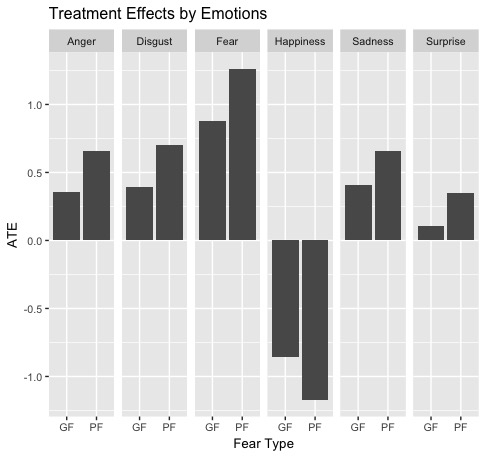
\includegraphics[scale=0.4]{Fig1.png}
\caption{The bar graphs show that fear treatments elicits positive change in related emotions and has the opposite effect on happiness. The differences in emotions are significant which shows that the treatment was able to successfully manipulate people's emotions.}
\centering
\end{figure}
    }        

    \frame{
        \frametitle{Replication}
\begin{table}[!htbp] \centering 
  \caption{Fear Treatment Reduces Dissent} 
  \label{ATEfeardissent} 
\scalebox{0.8}{\begin{tabular}{@{\extracolsep{5pt}}lcccc} 
\\[-1.8ex]\hline 
\hline \\[-1.8ex] 
 & \multicolumn{2}{c}{Hypothetical} & \multicolumn{2}{c}{Behavioral} \\ 
 \hline \\[-1.8ex]
\\[-1.8ex] & General Fear & Political Fear & General Fear & Political Fear\\ 
\\[-1.8ex] & (1) & (2) & (3) & (4)\\ 
\hline \\[-1.8ex] 
ATEs & -0.545 & -0.773 & -0.104 & -0.189 \\ 
SE & (0.077) & (0.080) & (0.050) & (0.053) \\
RI p-value & $<$ 0.001 & $<$ 0.001 & 0.03521 & 0.00016 \\ 
N & 484 & 486 & 329 & 326 \\ 
Sample & \multicolumn{2}{c}{All} & \multicolumn{2}{c}{Wristband} \\
\hline 
\hline \\[-1.8ex] 
\end{tabular}}
\begin{tablenotes}
      \small
\item Notes: The first row presents the estimated Average Treatment Effects (ATEs) of the general and political fear treatments in the hypothesis measure of propensity to dissent in Columns 1-2, and the behavioral measure in Columns 3-4. ATEs are calculated based on assignment to treatment and weighted by inverse propensity scores by block.
\end{tablenotes}
\end{table}     
    }
    \frame{
        \frametitle{Replication}
    \begin{figure}[!htbp]
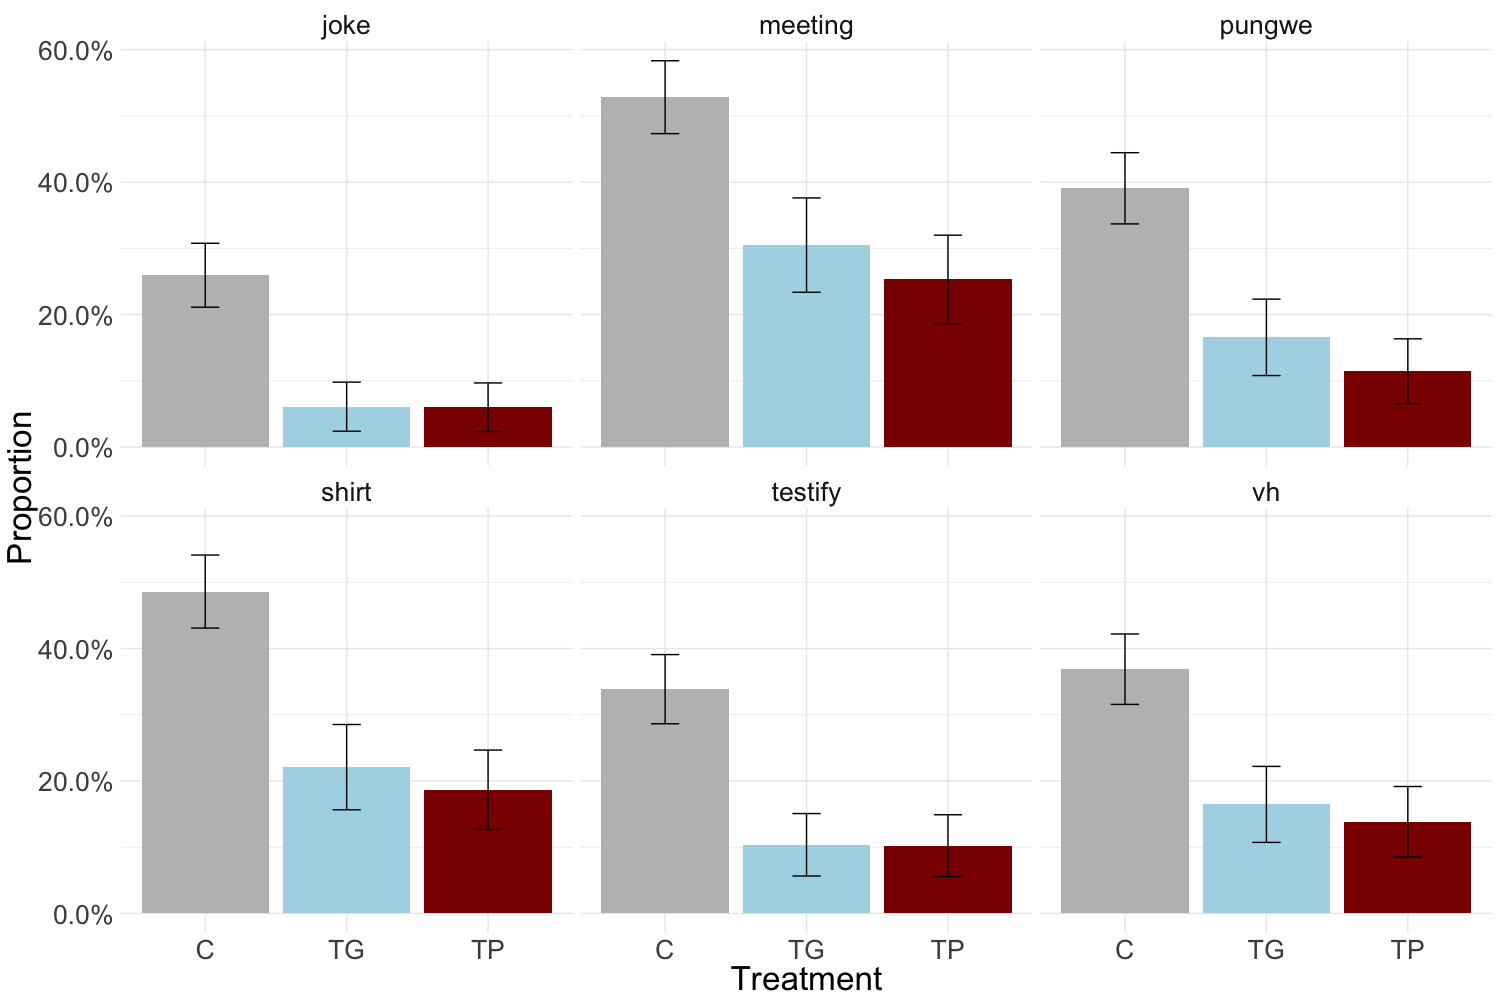
\includegraphics[scale=0.15]{Figure_2_Replicated.png}
\caption{The Fear Treatments Cause Substantively Large Increases in the Proportion of
Respondents Who Are Very Likely or Sure to Dissent During an Election Period}
\centering
\end{figure}
    }
    \frame{
        \frametitle{Replication}
    \begin{table}[!htbp] \centering 
  \caption{The Fear Treatments Increase Pessimism and Risk Aversion} 
  \label{feartreatmentmechanism} 
\scalebox{0.65}{\begin{tabular}{@{\extracolsep{5pt}}lcccccc} 
\hline \\[-1.8ex] 
\\[-1.8ex] & \multicolumn{2}{c}{Propensity of others to dissent} & \multicolumn{2}{c}{Perceived risk of repression} & \multicolumn{2}{c}{Risk aversion} \\ 
\\[-1.8ex] & General fear & Political fear & General fear & Political fear & General fear & Political fear \\ 
\\[-1.8ex] & (1) & (2) & (3) & (4) & (5) & (6)\\ 
\hline \\[-1.8ex] 
ATEs & -0.323 & -0.447 & 0.206 & 0.511 & 0.21 & 0.347 \\ 
RI p-value & 0.00059 & 0 & 0.02498 & 0 & 0.02474 & 0.00029 \\ 
N & 485 & 487 & 484 & 485 & 496 & 502 \\ 
\hline \\[-1.8ex] 
\end{tabular}}
\begin{tablenotes}
      \small
\item Notes: The first row presents the estimated Average Treatment Effects (ATEs) of the general and political fear treatments on beliefs about the likelihood that other opposition supporters will engage in dissent in Columns 1-2, on the perceived likelihood of repression in Columns 3-4, and on risk aversion in Columns 5-6. ATEs are calculated based on assignment to treatment and weighted by inverse propensity scores by block.
\end{tablenotes}
\end{table} 
    }

    \frame{
        \frametitle{Extension}
\begin{figure}[!htbp]
\label{emotions}
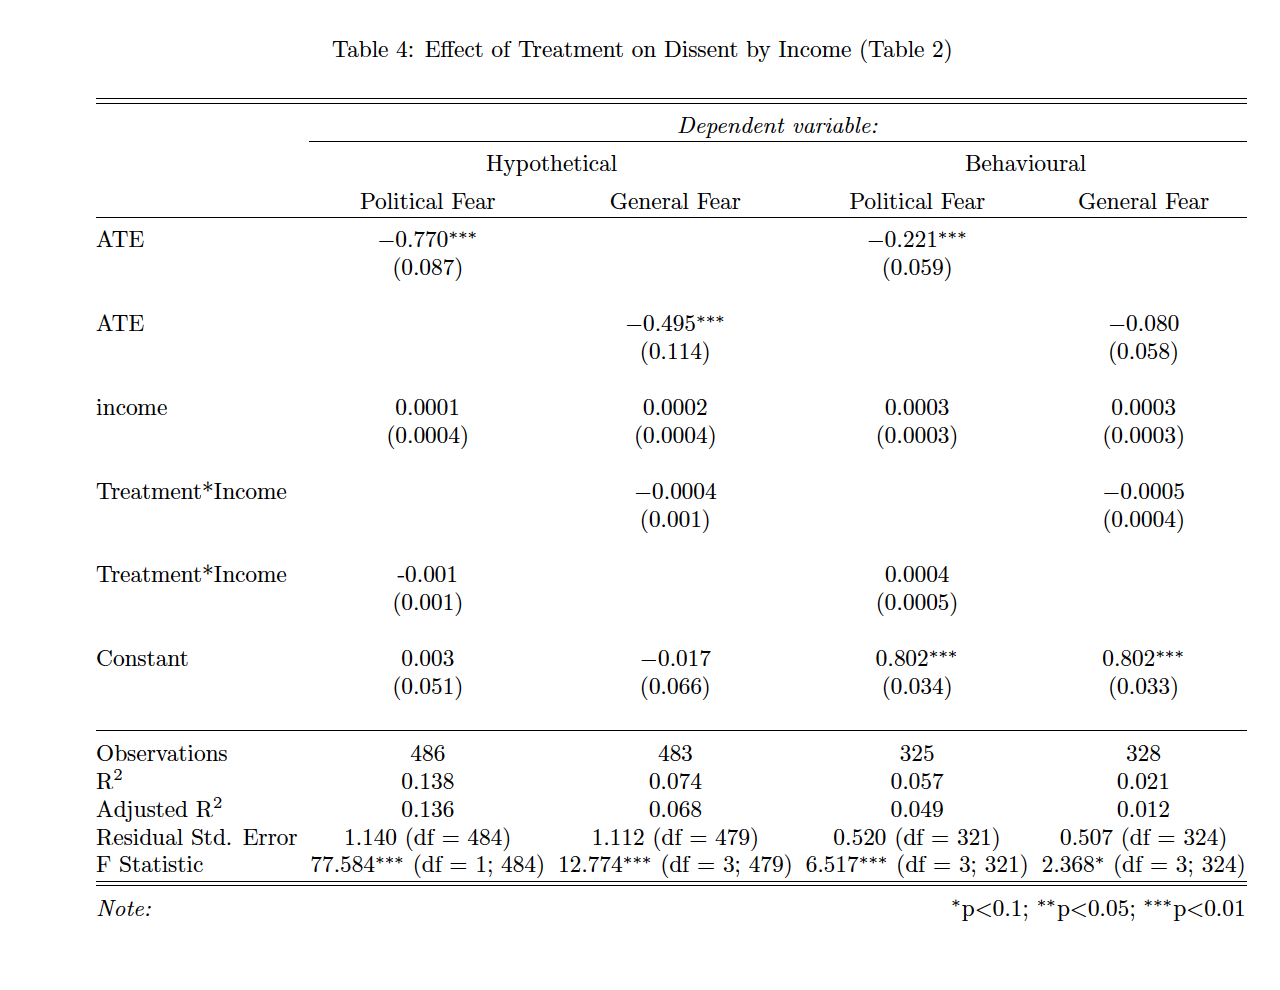
\includegraphics[scale=0.45]{Table_4.png}
\centering
\end{figure}

        }
    \frame{
        \frametitle{Extension}
\begin{figure}[!htbp]
\label{emotions}
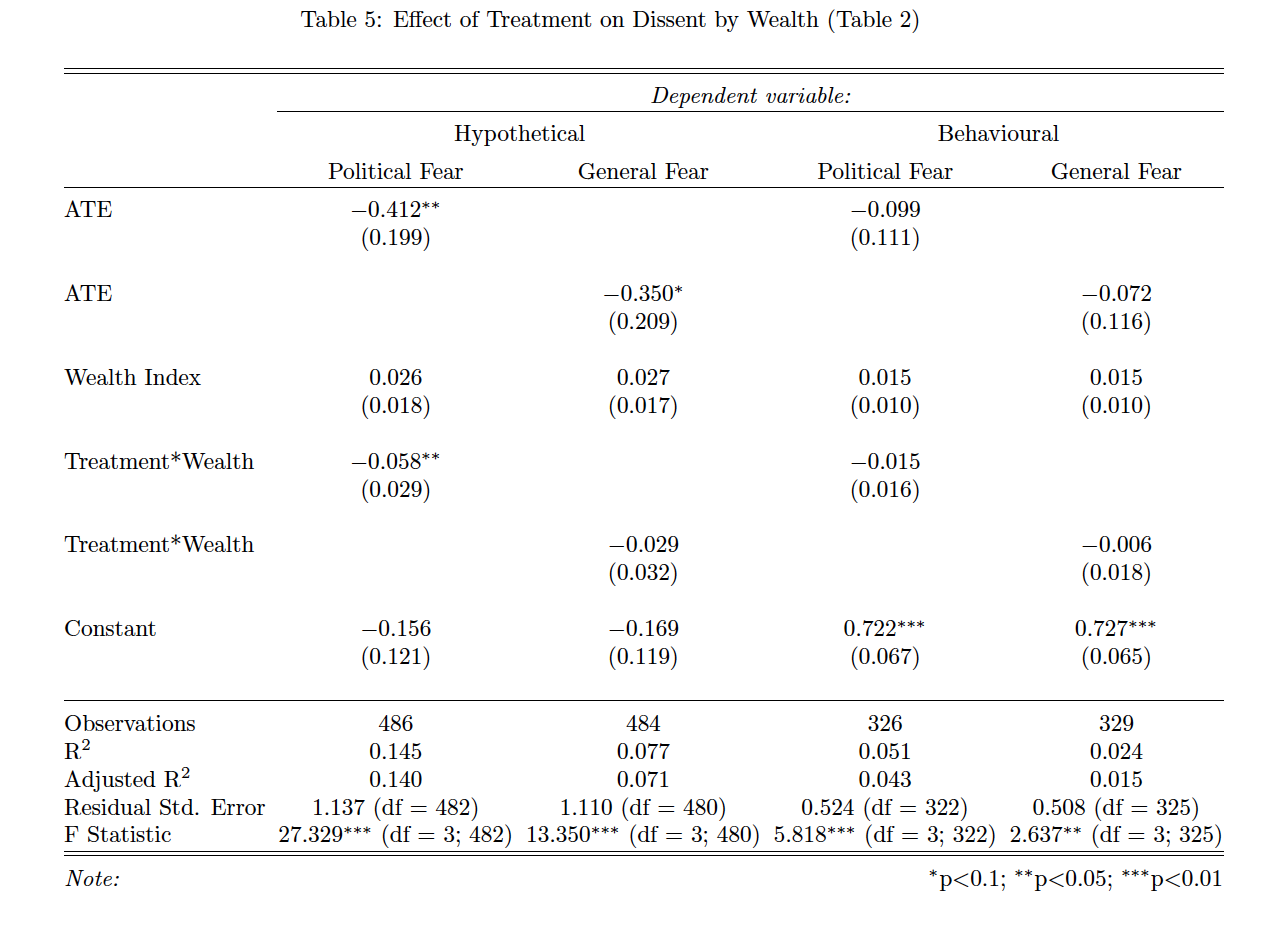
\includegraphics[scale=0.45]{Table_5.png}
\centering
\end{figure}   
        }
    \frame{
    \frametitle{Extension}
\begin{figure}[!htbp]
\label{emotions}
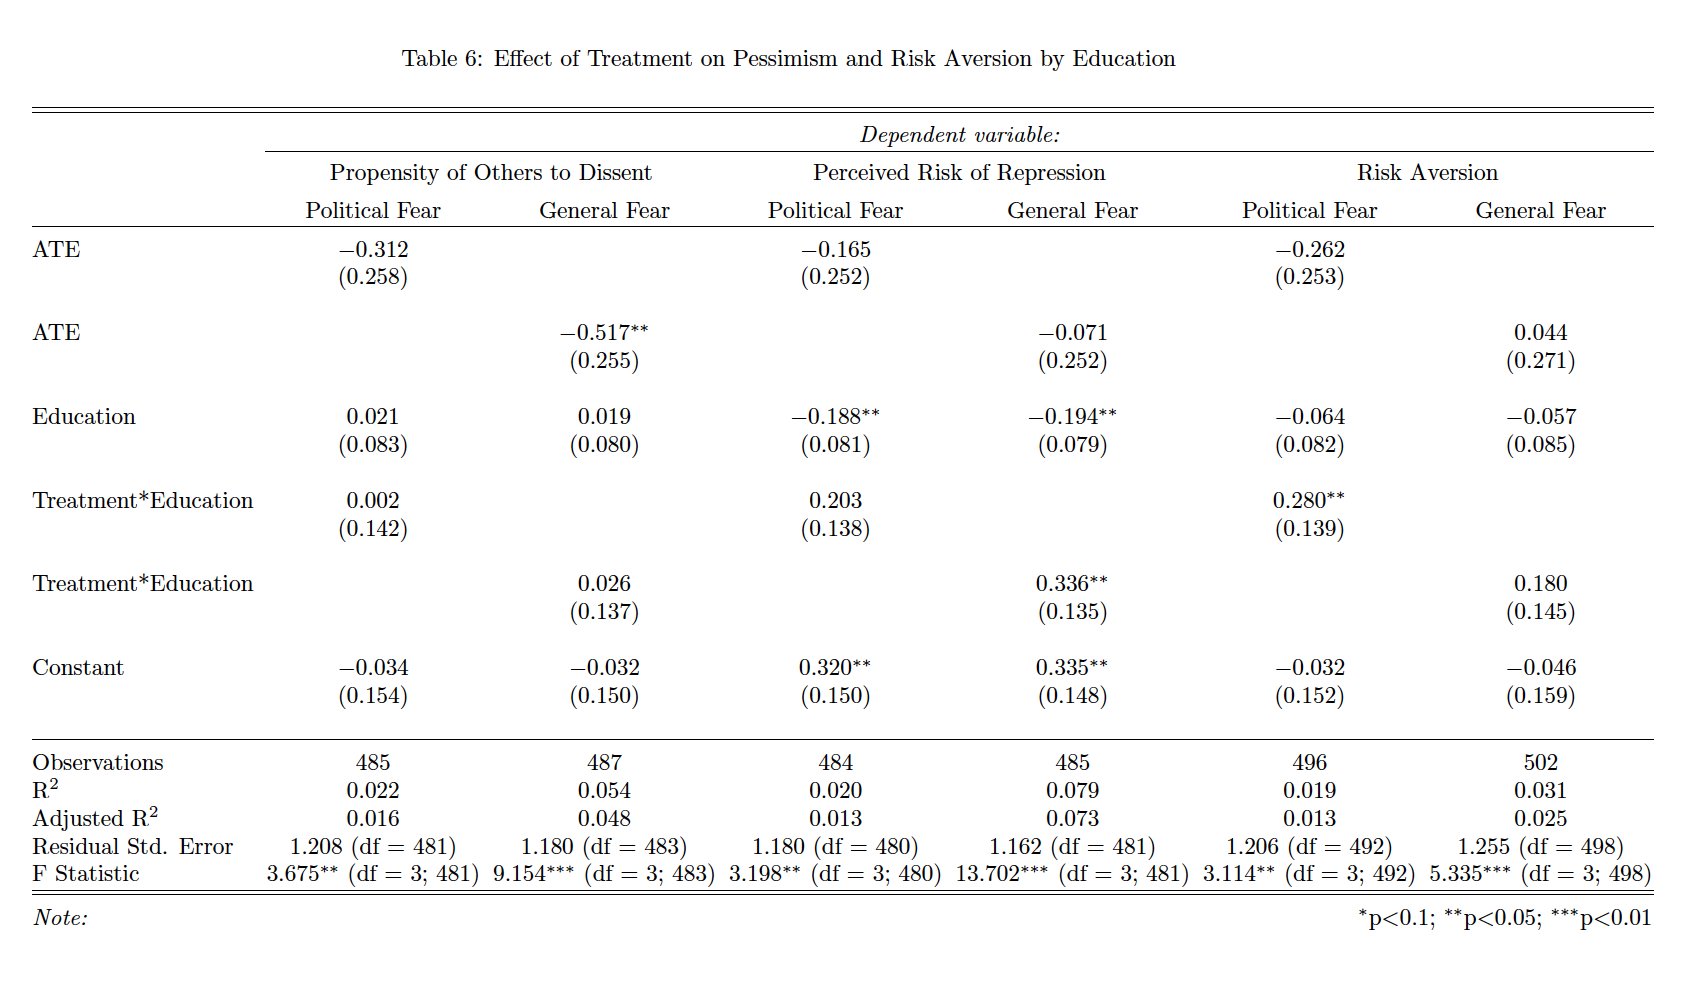
\includegraphics[scale=0.40]{Table_6.png}
\centering
\end{figure}  
        }
    \frame{
        \frametitle{Extension}
\begin{figure}[!htbp]
\label{emotions}
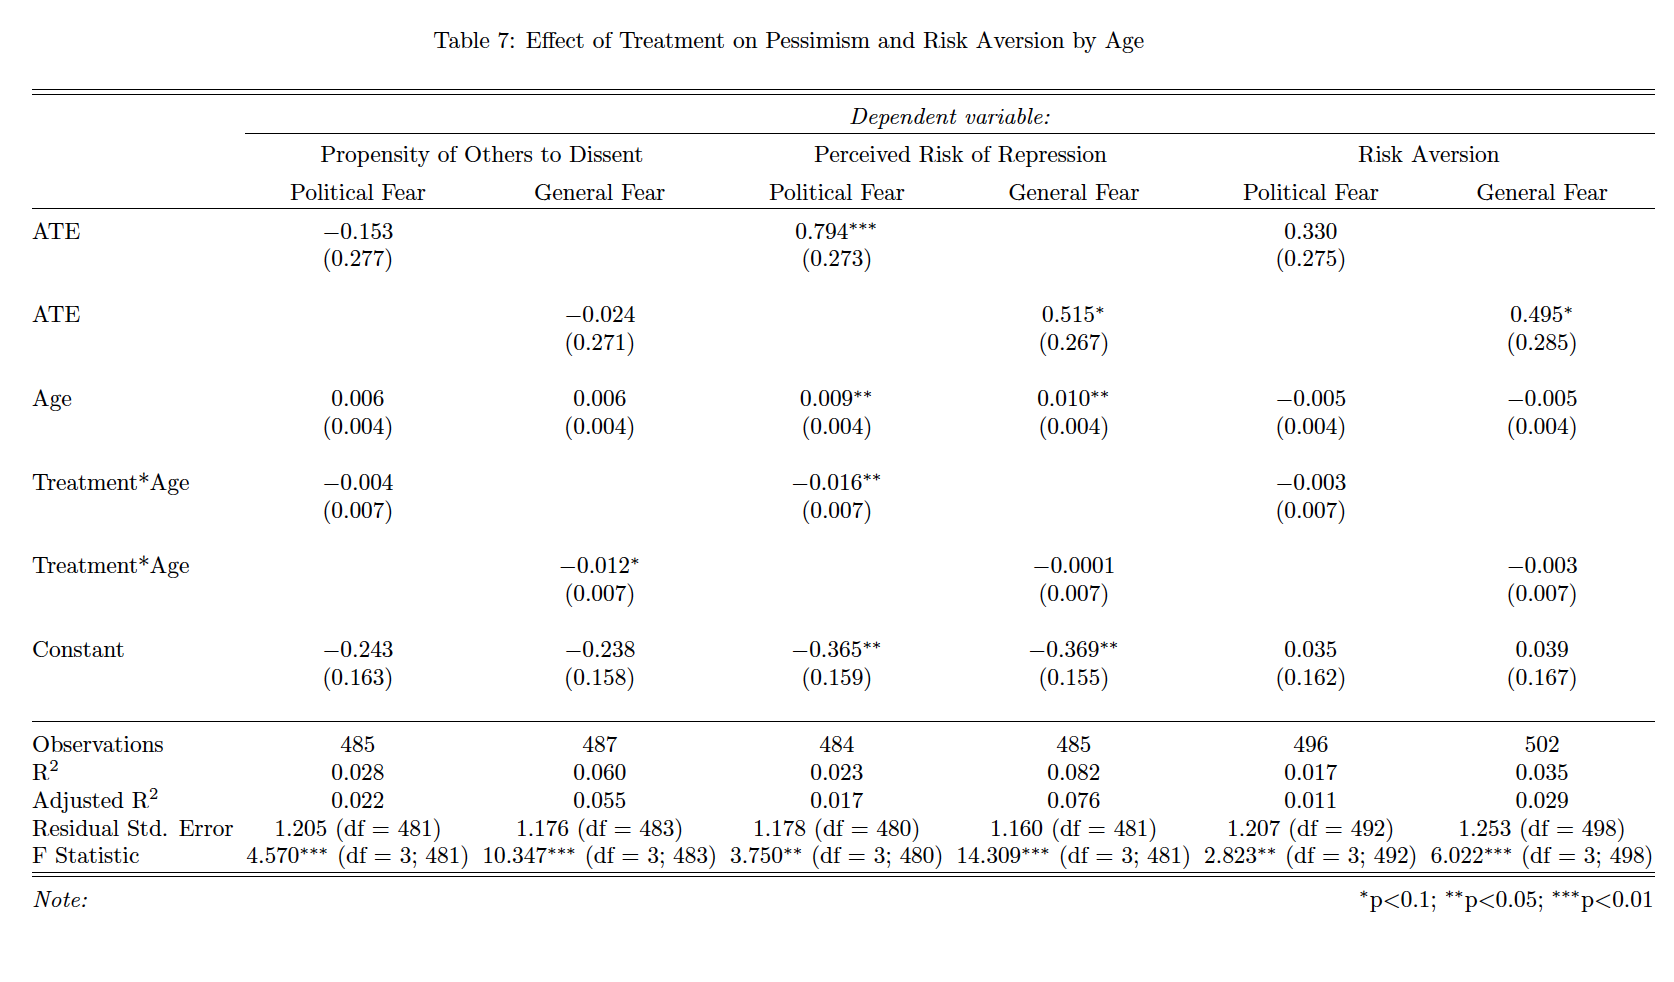
\includegraphics[scale=0.40]{Table_7.png}
\centering
\end{figure}  
        }
\frame{
    \frametitle{Extension}
\begin{figure}[!htbp]
\label{emotions}
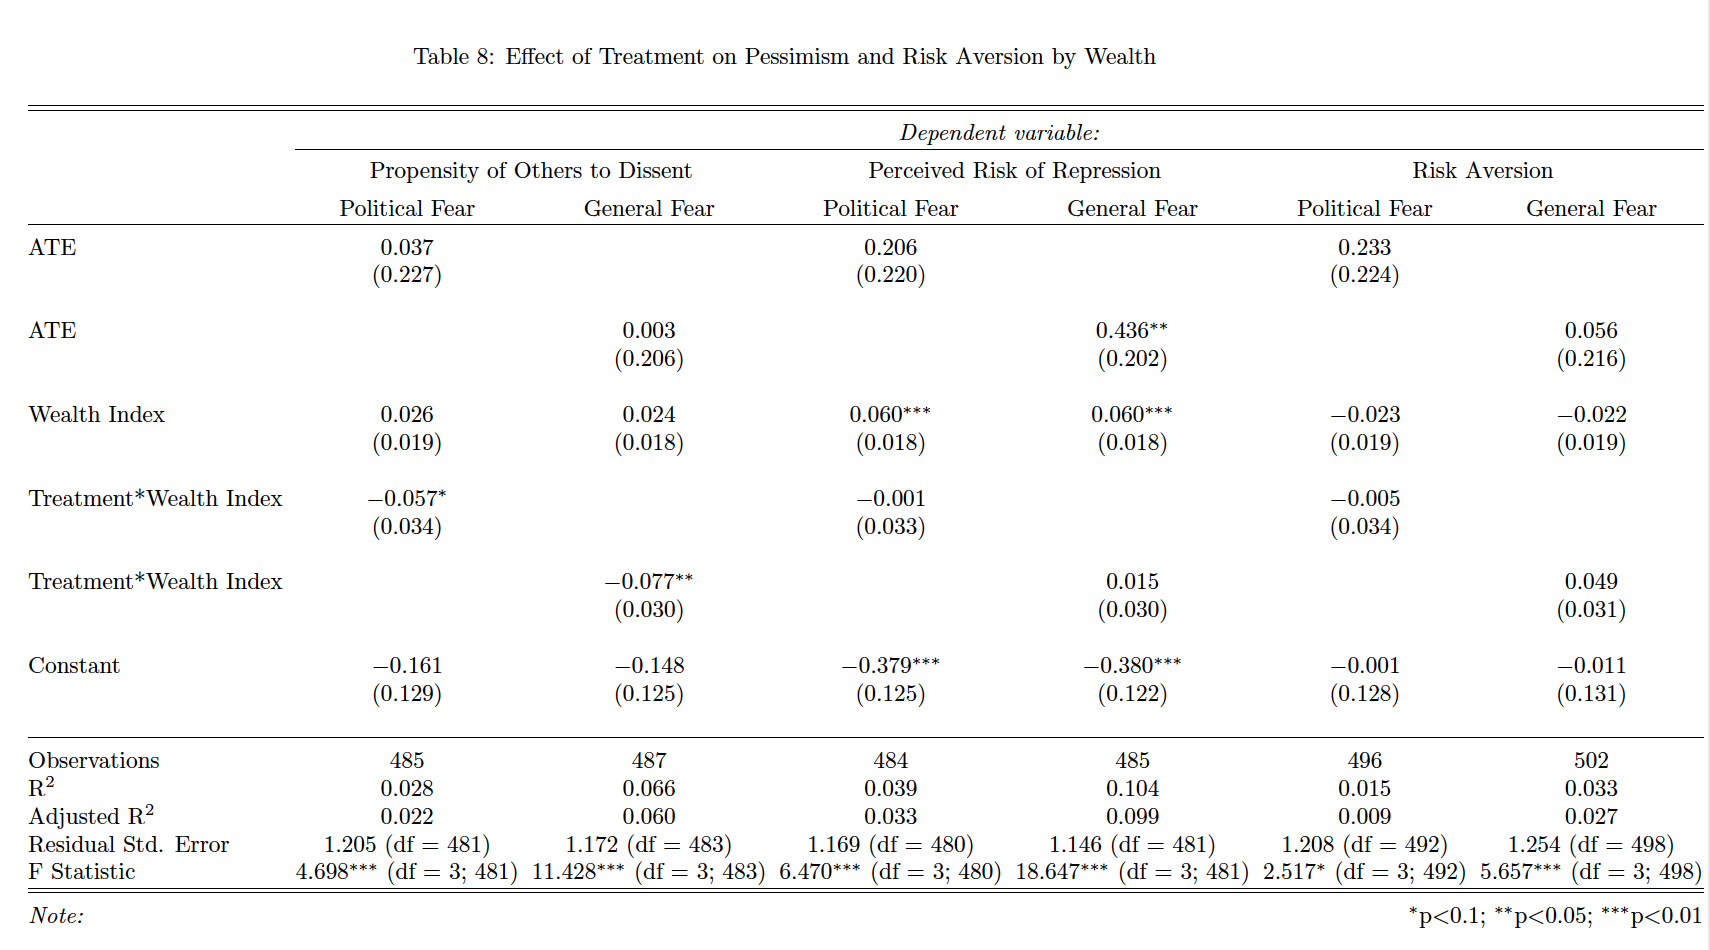
\includegraphics[scale=0.38]{Table_8.png}
\centering
\end{figure}  
}
\end{document}

